\documentclass[conference,10pt]{IEEEtran}
% BenchFuzz paper (v0.4). Every number is a macro from generated/results.tex and every results table is
% generated/tab_*.tex, both written by tools/compare_literature.py from the experiment logs.
\usepackage[T1]{fontenc}
\usepackage[utf8]{inputenc}
\usepackage{microtype}
\usepackage{graphicx}
\usepackage{booktabs}
\usepackage{tabularx}
\usepackage{multirow}
\usepackage{amsmath,amssymb}
\usepackage{amsfonts}
\usepackage{xcolor}
\usepackage{url}
\usepackage{tikz}
\usetikzlibrary{arrows.meta,positioning,fit,calc}
\usepackage[hidelinks]{hyperref}

% generated by tools/compare_literature.py -- do not edit
\newcommand{\BugBudget}{1,000}
\newcommand{\BugCount}{15}
\newcommand{\BugMutationAll}{13}
\newcommand{\BugMutationAny}{13}
\newcommand{\BugMutationRunRate}{86.7}
\newcommand{\BugRandomAll}{13}
\newcommand{\BugRandomAny}{14}
\newcommand{\BugRandomRunRate}{88.0}
\newcommand{\CovBest}{64.62}
\newcommand{\CovFalseAlarms}{0}
\newcommand{\CovHybridRandCi}{0.06}
\newcommand{\CovHybridRandInsnPerS}{132}
\newcommand{\CovHybridRandMean}{64.21}
\newcommand{\CovHybridRandPlateau}{227}
\newcommand{\CovHybridRandProgPerS}{3.9}
\newcommand{\CovHybridRandUnion}{3022}
\newcommand{\CovMutationCi}{0.08}
\newcommand{\CovMutationInsnPerS}{371}
\newcommand{\CovMutationMean}{64.57}
\newcommand{\CovMutationPlateau}{227}
\newcommand{\CovMutationProgPerS}{3.7}
\newcommand{\CovMutationUnion}{3039}
\newcommand{\CovN}{10,000}
\newcommand{\CovRandomCi}{0.00}
\newcommand{\CovRandomInsnPerS}{186}
\newcommand{\CovRandomMean}{63.79}
\newcommand{\CovRandomPlateau}{133}
\newcommand{\CovRandomProgPerS}{5.6}
\newcommand{\CovRandomUnion}{3000}
\newcommand{\CovSeeds}{7}
\newcommand{\CovTotalPrograms}{210,000}
\newcommand{\CovUniverse}{4,703}
\newcommand{\DdminOneMinimalPct}{100}
\newcommand{\DdminTestsMedian}{6}
\newcommand{\EOneBugs}{15}
\newcommand{\EOneDetected}{14}
\newcommand{\EOneLocHit}{14}
\newcommand{\EOnePrimaryHit}{9}
\newcommand{\ETwoFiveInjected}{5}
\newcommand{\ETwoFiveIsolated}{5}
\newcommand{\ETwoTrioInjected}{3}
\newcommand{\ETwoTrioIsolated}{3}
\newcommand{\EzCascadeInsns}{1,599}
\newcommand{\EzCascadeMatched}{150}
\newcommand{\EzCascadePrograms}{50}
\newcommand{\EzCascadeRuns}{150}
\newcommand{\EzGoldenInsns}{1,599}
\newcommand{\EzGoldenMatched}{150}
\newcommand{\EzGoldenPrograms}{50}
\newcommand{\EzGoldenRuns}{150}
\newcommand{\EzMasterCommit}{ef203c2}
\newcommand{\EzMasterInsns}{1,599}
\newcommand{\EzMasterMatched}{150}
\newcommand{\EzMasterPrograms}{50}
\newcommand{\EzMasterRuns}{150}
\newcommand{\EzProbeActual}{256}
\newcommand{\EzProbeExpected}{257}
\newcommand{\EzProbeInsn}{lb x3, 1(x1)}
\newcommand{\FenceRdMutationAttributed}{9}
\newcommand{\FenceRdMutationDet}{9}
\newcommand{\FenceRdMutationPrograms}{872}
\newcommand{\FenceRdMutationRuns}{10}
\newcommand{\FenceRdMutationTotal}{14,692}
\newcommand{\FenceRdRandomAttributed}{0}
\newcommand{\FenceRdRandomDet}{0}
\newcommand{\FenceRdRandomPrograms}{--}
\newcommand{\FenceRdRandomRuns}{10}
\newcommand{\FenceRdRandomTotal}{30,000}
\newcommand{\HddBugs}{14}
\newcommand{\HddCases}{80}
\newcommand{\HddCycRedMedian}{86.2}
\newcommand{\HddFewerTests}{29}
\newcommand{\HddLenRedMedian}{93.1}
\newcommand{\HddMinMedian}{3}
\newcommand{\HddOneMinimalPct}{100}
\newcommand{\HddOrigMedian}{36}
\newcommand{\HddSameSize}{73}
\newcommand{\HddSliceKept}{67}
\newcommand{\HddSmaller}{4}
\newcommand{\HddTestsMedian}{7}
\newcommand{\MixBenchALUImm}{45.4}
\newcommand{\MixBenchALUReg}{11.5}
\newcommand{\MixBenchBranch}{6.9}
\newcommand{\MixBenchJump}{1.5}
\newcommand{\MixBenchLUIAUIPC}{20.0}
\newcommand{\MixBenchLoad}{4.9}
\newcommand{\MixBenchMULDIV}{5.4}
\newcommand{\MixBenchStore}{4.4}
\newcommand{\MixRunCALUIMM}{57.5}
\newcommand{\MixRunCALUREG}{17.3}
\newcommand{\MixRunCBRANCH}{8.2}
\newcommand{\MixRunCJUMP}{2.0}
\newcommand{\MixRunCLOAD}{4.5}
\newcommand{\MixRunCLUIAUIPC}{2.2}
\newcommand{\MixRunCMULDIV}{2.7}
\newcommand{\MixRunCSTORE}{5.5}
\newcommand{\PMutationHybridRand}{0.001}
\newcommand{\PRandomHybridRand}{0.001}
\newcommand{\PRandomMutation}{0.001}
\newcommand{\PSixMutationDet}{10}
\newcommand{\PSixMutationProgs}{4}
\newcommand{\PSixMutationProgsMax}{27}
\newcommand{\PSixMutationRuns}{10}
\newcommand{\PSixMutationSecs}{0.74}
\newcommand{\PSixRandomDet}{10}
\newcommand{\PSixRandomProgs}{2}
\newcommand{\PSixRandomProgsMax}{11}
\newcommand{\PSixRandomRuns}{10}
\newcommand{\PSixRandomSecs}{0.15}
\newcommand{\RepBugs}{14}
\newcommand{\RepHuntMismatches}{0}
\newcommand{\RepHuntPrograms}{18,000}
\newcommand{\RepInterfaceProven}{2,400}
\newcommand{\RepLintRecovered}{14}
\newcommand{\RepNoopRejected}{14}
\newcommand{\RepOracleAccepted}{14}
\newcommand{\RepOracleCorrect}{14}
\newcommand{\RepRejGrowPrefix}{0}
\newcommand{\RepRejLint}{0}
\newcommand{\RepRejPatchFormat}{0}
\newcommand{\RepRejReproducer}{269}
\newcommand{\RepRejSuiteGate}{5}
\newcommand{\RepTplAccepted}{9}
\newcommand{\RepTplCertified}{7}
\newcommand{\RepTplCorrect}{9}
\newcommand{\RepTplExact}{4}
\newcommand{\RepTplHeldOutButWrong}{1}
\newcommand{\RepTplInterfaceOnly}{1}
\newcommand{\RepTplNotProven}{2}
\newcommand{\RepTplOverfit}{0}
\newcommand{\RepTplTriedMedian}{15}
\newcommand{\RepTplWitnessed}{1}
\newcommand{\RunCGemAccepted}{5}
\newcommand{\RunCGemAttempts}{133}
\newcommand{\RunCGemRejected}{126}
\newcommand{\RunCIters}{552}
\newcommand{\RunCLine}{61.75}
\newcommand{\RunCLlmCalls}{82}
\newcommand{\RunCMatch}{99.8}
\newcommand{\RunCRepairs}{4}
\newcommand{\RunCSeconds}{1,316}
\newcommand{\RunCToggle}{61.87}
\newcommand{\SynDsp}{4}
\newcommand{\SynFfPct}{0.09}
\newcommand{\SynFfs}{945}
\newcommand{\SynLutPct}{0.29}
\newcommand{\SynLutram}{6}
\newcommand{\SynLuts}{1,502}
\newcommand{\TierLOneMutationProgs}{2}
\newcommand{\TierLOneMutationSecs}{1.00}
\newcommand{\TierLOneRandomProgs}{2}
\newcommand{\TierLOneRandomSecs}{0.94}
\newcommand{\TierLThreeMutationProgs}{3}
\newcommand{\TierLThreeMutationSecs}{0.62}
\newcommand{\TierLThreeRandomProgs}{2}
\newcommand{\TierLThreeRandomSecs}{0.75}
\newcommand{\TierLTwoMutationProgs}{1}
\newcommand{\TierLTwoMutationSecs}{0.55}
\newcommand{\TierLTwoRandomProgs}{1}
\newcommand{\TierLTwoRandomSecs}{0.50}
\newcommand{\TputCascade}{2,489}
\newcommand{\TputDifuzzRTLWithFPGA}{728}
\newcommand{\TputSoloMutation}{1,114}
\newcommand{\TputSoloRandom}{544}
\newcommand{\TputTurboFuzz}{309,676}
\newcommand{\UniAlwaysMissing}{fence, jalr}
\newcommand{\UniHybridRandCFunc}{98.02}
\newcommand{\UniHybridRandCISS}{89.83}
\newcommand{\UniHybridRandCLine}{65.03}
\newcommand{\UniHybridRandCToggle}{64.18}
\newcommand{\UniHybridRandCU}{79.26}
\newcommand{\UniIssStatements}{118}
\newcommand{\UniMutationCFunc}{96.35}
\newcommand{\UniMutationCISS}{89.83}
\newcommand{\UniMutationCLine}{65.03}
\newcommand{\UniMutationCToggle}{64.70}
\newcommand{\UniMutationCU}{78.98}
\newcommand{\UniRandomCFunc}{98.02}
\newcommand{\UniRandomCISS}{89.83}
\newcommand{\UniRandomCLine}{65.03}
\newcommand{\UniRandomCToggle}{63.74}
\newcommand{\UniRandomCU}{79.15}
\newcommand{\UniWeights}{0.25, 0.25, 0.25, 0.25}
\newcommand{\UniqHybridRandNotMutation}{0}
\newcommand{\UniqHybridRandNotRandom}{22}
\newcommand{\UniqMutationNotHybridRand}{17}
\newcommand{\UniqMutationNotRandom}{39}
\newcommand{\UniqRandomNotHybridRand}{0}
\newcommand{\UniqRandomNotMutation}{0}
\newcommand{\UnrLinePoints}{180}
\newcommand{\UnrLineUnreached}{64}
\newcommand{\UnrOther}{0}
\newcommand{\UnrRegions}{53}
\newcommand{\UnrToggleBits}{4,112}
\newcommand{\UnrToggleUnreached}{1,485}


\newcommand{\code}[1]{\texttt{\detokenize{#1}}}
\newcommand{\figpdf}[2]{\IfFileExists{#1}{\includegraphics[width=#2]{#1}}{\fbox{\parbox{#2}{\centering\scriptsize missing \detokenize{#1}}}}}
\newcommand{\gen}[1]{\IfFileExists{generated/#1}{\input{generated/#1}}{\emph{(table not generated)}}}
\newcommand{\RQ}[1]{\textbf{RQ#1}}
\tikzset{
  blk/.style={draw,rounded corners=2pt,align=center,font=\scriptsize,inner sep=2.5pt,minimum height=7mm},
  sw/.style={blk,fill=green!10}, hw/.style={blk,fill=orange!14}, gen/.style={blk,fill=blue!8},
  llm/.style={blk,fill=purple!10}, ana/.style={blk,fill=gray!12},
  arr/.style={-{Stealth[length=1.6mm]},semithick}, zone/.style={draw,dashed,rounded corners=3pt,inner sep=3pt},
}

\begin{document}

\title{BenchFuzz: Lockstep Differential Fuzzing, Hierarchical Delta Debugging and Guarded Repair for RISC-V RTL\\
\large A Controlled Study on PicoRV32 and a Roadmap to FPGA Acceleration}

\author{\IEEEauthorblockN{Subodh Satish Dalvi}
\IEEEauthorblockA{School of Electrical and Computer Engineering, The University of Sydney\\
Draft v0.4 --- October 2026}}

\maketitle

\begin{abstract}
Processor verification spends most of its effort on generating stimulus, deciding whether the design misbehaved, and turning a
long failing test into something a designer can act on. Recent LLM-guided fuzzers such as ChipFuzzer report large gains in condition
coverage and bug detection, but they evaluate coverage and bug finding without minimisation or repair, on different designs, metrics and
budgets, which makes their numbers hard to transfer. We present BenchFuzz, a role-separated differential verification loop for RISC-V
cores, and a controlled study of it on PicoRV32. An immutable Python RV32IM reference and Verilator-compiled RTL are compared at every
retirement through the RISC-V Formal Interface; failures are sliced with architectural state preloading and minimised by flat and
hierarchical delta debugging; candidate RTL patches pass lint, reproducer, prefix-growth and whole-suite gates before acceptance. On
unmodified YosysHQ PicoRV32 the oracle produces no false alarm in \EzMasterMatched{} of \EzMasterRuns{} control runs and settles the
long-open \code{mem_addr} discrepancy as a presentation-convention gap. The same harness reproduces Cascade's PicoRV32 bug P6
(CVE-2023-34899) on the commit Cascade evaluated, both with a directed probe and with blind fuzzing in a median of \PSixRandomProgs{}
programs, and its mutation fuzzer exposes a residual specification deviation on current master: a \code{fence} with a non-zero
reserved \code{rd} field writes zero to that register. Across \CovSeeds{} seeds per method, constrained-random and coverage-guided mutational fuzzing saturate every reachable RTL line of
the RV32IM configuration within a few hundred programs; all \UnrLineUnreached{} unreached line points are configuration-dead or outside
the ISA scope. Blind random fuzzing detects \BugRandomAny{} of the \BugCount{} injected bugs, three tiers from bit-level operator faults to an
intermittent bus-protocol fault, while one literal mutation from the original brief is equivalent on every valid program. Delta debugging
reduces fuzzer-found failures by a median \HddLenRedMedian\% in length and \HddCycRedMedian\% in cycles. Positive and negative
controls confirm that the repair gates accept correct patches and reject wrong ones. A spectrum-ranked template-repair baseline without
an LLM produces gate-passing patches for \RepTplAccepted{} of \RepBugs{} observable bugs, but whole-core formal equivalence certifies only
\RepTplCertified: one accepted patch is wrong for rare operands and another changes an output the lockstep oracle never observes,
although both passed every regression and held-out test. We tabulate the published results of ChipFuzzer, Cascade,
TheHuzz, TurboFuzz, BMCFuzz and Encarsia with their sources, state precisely which comparisons are and are not meaningful, and give a
measured-resource roadmap for moving the loop onto a Zynq UltraScale+ SoC following TurboFuzz.
\end{abstract}

\begin{IEEEkeywords}
hardware fuzzing, RISC-V, differential testing, delta debugging, automated program repair, LLM, FPGA
\end{IEEEkeywords}

%% =====================================================================
\section{Introduction}
%% =====================================================================
Pre-silicon verification is the most expensive phase of processor design, often cited at over 70\% of project effort~\cite{chipfuzzer}.
Hardware fuzzers~\cite{rfuzz,difuzzrtl,thehuzz,cascade} generate instruction streams, run them on RTL and compare against an ISA model.
LLM-based generators~\cite{chipfuzzer} now steer generation toward uncovered code, and FPGA-resident fuzzers~\cite{turbofuzz} remove
the simulation bottleneck. Three gaps motivate this work.

\emph{(i) Oracle soundness is rarely measured.} A differential oracle that disagrees with correct RTL for a convention reason (for
example, how a load's address is presented) produces false alarms that the rest of the pipeline then tries to ``debug''. Our own earlier
prototype did exactly that.

\emph{(ii) Detection is where most evaluations stop.} Failing programs from fuzzers are long; Cascade prunes them~\cite{cascade}, but
minimisation and repair are rarely evaluated together with detection.

\emph{(iii) Published numbers do not transfer.} Results are reported on different cores, coverage definitions (condition,
mux-toggle, register-toggle), budgets and reference simulators, so a table that places them side by side with a new tool can mislead.

\paragraph*{Contributions}
\begin{itemize}
  \item A \textbf{role-separated architecture} (Sec.~\ref{sec:arch}) in which only one component may write the RTL, the reference model
        is immutable, and every LLM output passes through a validator or a patch gate.
  \item A \textbf{measured control on unmodified upstream RTL} (Sec.~\ref{sec:rq1}): zero false alarms on YosysHQ master and on the
        commit used by Cascade, and a resolution of the \code{mem_addr} 2019/2016 discrepancy as a convention gap.
  \item A \textbf{reproduction of a published bug}, Cascade P6, on the same DUT commit, and a \textbf{residual FENCE deviation} on
        current upstream master found by mutational fuzzing (Sec.~\ref{sec:p6}).
  \item A \textbf{15-bug, three-tier injection suite} with observability checks, including a mutant that is equivalent on all valid programs and an intermittent
        bus fault (Sec.~\ref{sec:bugs}).
  \item \textbf{Head-to-head coverage and time-to-bug benchmarks} with seven to ten seeds, confidence intervals and Mann--Whitney tests on one
        harness (Secs.~\ref{sec:rq2}--\ref{sec:rq3}), and a classification of everything left uncovered.
  \item \textbf{Hierarchical delta debugging} over basic blocks and instructions, evaluated against flat ddmin on fuzzer-found failures
        with a 1-minimality check (Sec.~\ref{sec:rq4}).
  \item \textbf{Guard validation for LLM repair} with positive and negative controls, a CirFix-style template baseline ranked by
        Ochiai suspiciousness, \textbf{formal certification} of accepted patches that exposes a gate-passing, held-out-passing but wrong
        patch, and an independent-sample pass@$k$ harness (Sec.~\ref{sec:rq5}).
  \item A \textbf{unified co-coverage metric} with explicit weights and a demonstration of why components must be reported
        (Sec.~\ref{sec:rq6}); a \textbf{sourced comparison} with six published systems (Sec.~\ref{sec:sota}); and an \textbf{FPGA
        roadmap} with measured resource figures (Sec.~\ref{sec:fpga}).
\end{itemize}

%% =====================================================================
\section{Background and Related Work}\label{sec:background}
%% =====================================================================
\paragraph*{Processor fuzzing} RFUZZ~\cite{rfuzz} brought coverage-guided mutation to RTL; DifuzzRTL~\cite{difuzzrtl} added
control-register coverage; TheHuzz~\cite{thehuzz} used golden-model comparison and reached coverage 1.98$\times$ faster than random
regression and 3.33$\times$ faster than DifuzzRTL on four cores, finding 11 bugs. Cascade~\cite{cascade} generates long programs whose
control flow is entangled with their data flow so that a correct CPU always terminates; it reports the same coverage 28.2$\times$ and
97$\times$ faster than TheHuzz and DifuzzRTL and 37 new bugs (29 CVEs) in five of six cores, among them six in PicoRV32 (CSR, counter
and \code{fence} handling). BMCFuzz~\cite{bmcfuzz} combines bounded model checking with fuzzing. Encarsia~\cite{encarsia} injects
realistic bugs into CPU netlists to evaluate fuzzers fairly, one bug per design copy.

\paragraph*{LLM-guided fuzzing} ChipFuzzer~\cite{chipfuzzer} (preprint) selects uncovered RTL lines, retrieves the seed with the most
similar control-flow path, asks an LLM for an assembly test with a discrepancy analysis, and corrects syntax and semantics in at most five
rounds each; a bug-guided stage mines 128 historical bug fixes. On RocketCore, BOOM and CVA6 it reports condition coverage 9.1, 1.2 and
7.0 points above the strongest baseline after 24\,h, and 61.1\% of 90 Encarsia bugs against 36.7--40\%. Its ablation is instructive: an
LLM without guidance reaches 61.4\% condition coverage and finds no bug.

\paragraph*{Acceleration} TurboFuzz~\cite{turbofuzz} (preprint) moves generation, execution, checking and coverage onto one Zynq
UltraScale+ SoC and reports 309{,}676 executed instructions per second against 2{,}489 for Cascade and 728 for FPGA-assisted DifuzzRTL.

\paragraph*{Debugging and repair} Delta debugging~\cite{ddmin} minimises failure-inducing inputs; HDD~\cite{hdd} applies it level by
level over a tree. Spectrum-based fault localisation (Ochiai~\cite{ochiai}) ranks code by correlation with failing runs. CirFix~\cite{cirfix}
repairs Verilog by template search guided by simulation. pass@$k$~\cite{codex} measures sampled code generation.

%% =====================================================================
\section{System Architecture}\label{sec:arch}
%% =====================================================================
\begin{figure*}[t]
\centering
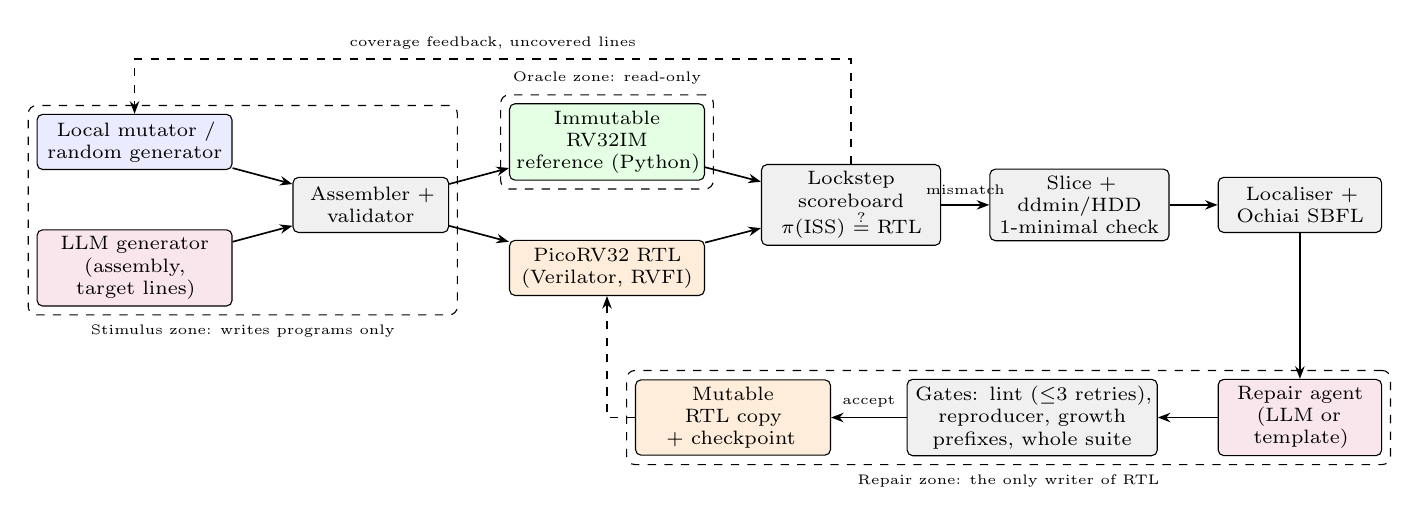
\begin{tikzpicture}[x=1cm,y=1cm]
% row 1 (y=1.6): stimulus -> oracle; row 0 (y=0): RTL; row -1.9: repair zone
\node[gen,text width=2.3cm] (mut)  at (0.0, 1.6) {Local mutator /\\random generator};
\node[llm,text width=2.3cm] (llmg) at (0.0, 0.0) {LLM generator\\(assembly, target lines)};
\node[ana,text width=1.8cm] (val)  at (3.0, 0.8) {Assembler +\\validator};
\node[sw,text width=2.3cm]  (iss)  at (6.0, 1.6) {Immutable RV32IM\\reference (Python)};
\node[hw,text width=2.3cm]  (rtl)  at (6.0, 0.0) {PicoRV32 RTL\\(Verilator, RVFI)};
\node[ana,text width=2.1cm] (sb)   at (9.1, 0.8) {Lockstep scoreboard\\$\pi$(ISS) $\stackrel{?}{=}$ RTL};
\node[ana,text width=2.1cm] (dd)   at (12.0, 0.8) {Slice + ddmin/HDD\\1-minimal check};
\node[ana,text width=1.9cm] (loc)  at (14.8, 0.8) {Localiser +\\Ochiai SBFL};
\node[llm,text width=1.9cm] (rep)  at (14.8,-1.9) {Repair agent\\(LLM or template)};
\node[ana,text width=3.0cm] (gate) at (11.4,-1.9) {Gates: lint ($\le$3 retries), reproducer, growth prefixes, whole suite};
\node[hw,text width=2.3cm]  (mrtl) at (7.6,-1.9) {Mutable RTL copy\\+ checkpoint};
\draw[arr] (mut) -- (val); \draw[arr] (llmg) -- (val);
\draw[arr] (val) -- (iss); \draw[arr] (val) -- (rtl);
\draw[arr] (iss) -- (sb); \draw[arr] (rtl) -- (sb);
\draw[arr] (sb) -- node[above,font=\tiny]{mismatch} (dd); \draw[arr] (dd) -- (loc); \draw[arr] (loc) -- (rep);
\draw[arr] (rep) -- (gate); \draw[arr] (gate) -- node[above,font=\tiny]{accept} (mrtl);
\draw[arr,dashed] (mrtl.west) -| (rtl.south);
\draw[arr,dashed] (sb.north) -- (9.1,2.65) -- node[above,font=\tiny]{coverage feedback, uncovered lines} (0,2.65) -- (mut.north);
\node[zone,fit=(mut)(llmg)(val)] (z1) {};
\node[font=\tiny,anchor=north] at (z1.south) {Stimulus zone: writes programs only};
\node[zone,fit=(iss)] (z2) {};
\node[font=\tiny,anchor=south] at (z2.north) {Oracle zone: read-only};
\node[zone,fit=(mrtl)(gate)(rep)] (z3) {};
\node[font=\tiny,anchor=north] at (z3.south) {Repair zone: the only writer of RTL};
\end{tikzpicture}
\caption{BenchFuzz workflow and role boundaries. Dashed boxes are trust zones; solid arrows carry data, dashed arrows feedback.}
\label{fig:arch}
\end{figure*}

Figure~\ref{fig:arch} shows the loop. Table~\ref{tab:roles} lists what each role may read and write. The boundaries are enforced in
code, not by convention: the reference model has no dependency on the harness; generators can only emit programs that the validator
accepts; patches are spliced only into the line ranges the localiser offered; and acceptance requires that the entire regression suite
match after the patch with no previously passing program failing.

\begin{table}[t]
\centering\scriptsize
\caption{Role-separated workflow boundaries.}\label{tab:roles}
\begin{tabularx}{\columnwidth}{@{}l X X@{}}
\toprule
Role & May read & May write\\
\midrule
Generators (random, mutation, LLM) & coverage summary, uncovered lines, corpus & programs (validated before use)\\
Reference model & program & retirement records only\\
RTL simulator & mutable RTL copy, program & RVFI trace, coverage\\
Scoreboard & both traces & verdict, first mismatch\\
Delta debugger & failing program, verdict oracle & reproducers\\
Localiser / SBFL & RTL text, coverage spectra & candidate blocks\\
Repair agent & offered blocks, reproducer, signature & block patches (text)\\
Gates & candidate RTL, suite & accept / reject; checkpoint in \code{logs/checkpoints/}\\
\bottomrule
\end{tabularx}
\end{table}

\paragraph*{Oracle} For program $p$ let $r_i^{\mathrm{ISS}}$ and $r_i^{\mathrm{RTL}}$ be the $i$-th retirement records (PC before and
after, instruction, destination register and value, memory address, masks and data). The verdict is
\begin{equation}
  \mathrm{ok}(p) \iff |R^{\mathrm{RTL}}| = |R^{\mathrm{ISS}}| \;\wedge\; \forall i:\; \pi\!\left(r_i^{\mathrm{ISS}}\right) = r_i^{\mathrm{RTL}},
\end{equation}
where $\pi$ applies the DUT's presentation convention. For PicoRV32 (riscv-formal~\cite{riscvformal} \code{ALIGNED_MEM}) $\pi$ replaces the architectural
address $a$ by $a \wedge \lnot 3$ and leaves the byte lane to the masks. Missing and extra retirements are failures, so a core that traps
early cannot pass by default. The DUT is built with \code{ENABLE_FAST_MUL}, \code{ENABLE_DIV} and \code{REGS_INIT_ZERO}; the validator
accepts exactly RV32IM plus \code{fence}.

%% =====================================================================
\section{Metrics}\label{sec:metrics}
%% =====================================================================
\paragraph*{RTL coverage} Let $P = P_{\mathrm{line}} \cup P_{\mathrm{tog}} \cup P_{\mathrm{br}}$ be the Verilator coverage points of the
build and $H(p) \subseteq P$ those hit by $p$. After $k$ programs
\begin{equation}
  C_k = \frac{\left|\bigcup_{j \le k} H(p_j)\right|}{|P|},\qquad C_k^{x} = \frac{\left|\bigcup_{j \le k} H(p_j) \cap P_x\right|}{|P_x|}.
\end{equation}
\paragraph*{Reference-model statement coverage} With $S$ the executable statements of the reference model and $S(p)$ those executed,
$C_{\mathrm{ISS}} = |\bigcup_j S(p_j)|/|S|$ ($|S| = \UniIssStatements$). Our reference is Python, so this replaces gcov on a C++ ISS.
\paragraph*{Functional coverage} Five covergroups $G_1..G_5$ with bins $B_g$ (49 mnemonics; 12 branch-type$\times$outcome bins; 20
load/store size$\times$byte-offset bins; 12 RV32M corner cases such as division by zero and signed overflow; 7 register-value
patterns): $C_{\mathrm{func}} = \frac{1}{5}\sum_g |\mathrm{hit}_g|/|B_g|$.
\paragraph*{Unified co-coverage}
\begin{equation}
  C_U = w_L C^{\mathrm{line}} + w_T C^{\mathrm{tog}} + w_S C_{\mathrm{ISS}} + w_F C_{\mathrm{func}},\quad \textstyle\sum w = 1,
\end{equation}
with equal weights ($\UniWeights$) unless stated. $C_U$ is a monitoring aggregate, not a validated predictor of bug finding; we always
report its components.
\paragraph*{Plateau and efficiency} Following ChipFuzzer, a run has plateaued at $k$ when $C_k - C_{k-100} < 0.1$ percentage points.
With $C^\ast$ the best final coverage over all runs, $N_\rho = \min\{k : C_k \ge \rho C^\ast\}$ is the number of programs needed to reach
a relative threshold $\rho$.
\paragraph*{Time-to-bug} $N_{\mathrm{bug}}$ is the index of the first program with $\neg\mathrm{ok}(p)$ on the buggy RTL; we also report
seconds, excluding the one-off Verilator build.
\paragraph*{Minimisation} For a failing $p$ and its minimised $p^\ast$: $R_{\mathrm{len}} = 1 - |p^\ast|/|p|$ (instructions) and
$R_{\mathrm{cyc}} = 1 - \mathrm{cyc}(p^\ast)/\mathrm{cyc}(p)$; $p^\ast$ is 1-minimal if removing any single unprotected instruction makes it pass.
\paragraph*{Suspiciousness} For RTL line $\ell$ with $e_f$ failing and $e_p$ passing runs executing it out of $F$ failing runs,
$\mathrm{Ochiai}(\ell) = e_f / \sqrt{F (e_f + e_p)}$.
\paragraph*{Repair} With $n$ independent samples and $c$ successes, $\mathrm{pass@}k = 1 - \binom{n-c}{k} / \binom{n}{k}$~\cite{codex}.

%% =====================================================================
\section{Bug Suite}\label{sec:bugs}
%% =====================================================================
Each bug is a list of exact-text edits applied to a fresh copy of the golden RTL (multi-edit bugs are applied in order; markers must be
unique). Table~\ref{tab:e1} lists the suite. Tier L1 contains signal and operator faults, L2 control and block faults, and L3 system and
protocol faults. Five legacy bugs come from the prototype; they contain conspicuous constants (for instance \code{latched_rd == 5}) that
an LLM can spot by reading, so ten plain mutations were added. Three items of the original brief needed refinement (details in
Appendix~\ref{app:brief}): the only AND operators in \code{picorv32_pcpi_fast_mul} are logical; mutating that decode term gives a mutant
that is equivalent on valid programs (Sec.~\ref{sec:rq3}), so we also add an observable signedness fault inside the same module and keep the bitwise AND$\rightarrow$OR in the ALU.
\code{mem_ready} is a testbench input, so the handshake fault is placed in the core's reaction to it, in a deterministic and an
intermittent (timing-gated) variant. Interrupt trap flags are unobservable with \code{ENABLE_IRQ=0} and no interrupt model in the
reference, so an uncleared \code{latched_branch} flag substitutes.

\begin{table}[t]
\centering\scriptsize
\caption{E1: bug suite, targeted stimulus, minimisation of the stimulus and localisation (Hit = an offered block contains the edit).}
\label{tab:e1}
\resizebox{\columnwidth}{!}{\gen{tab_e1.tex}}
\end{table}

%% =====================================================================
\section{Experimental Setup}\label{sec:setup}
%% =====================================================================
All experiments ran in WSL2 Ubuntu on an 8-core x86-64 laptop with 15\,GB RAM, Verilator 5.032 and Yosys 0.52, with the DUT at
YosysHQ master (\code{ef203c2}) unless stated. Generators: \emph{Random} (constrained-random RV32IM programs of 20 body instructions
over a pool of interesting values), \emph{Cov.-guided mutation} (an AFL-style corpus loop that keeps programs adding coverage and mutates
by bit flips outside the opcode, swaps, splices, immediate rewrites and fresh segments), and \emph{Hybrid} (mutation until the plateau rule
fires, then random, the equal-budget control for ChipFuzzer's plateau switch). These are re-implementations of strategies, not the
published tools. Budgets are counted in validated programs, the testcase unit of ChipFuzzer's Table~2, so results do not depend on
machine load: \CovN{} programs per coverage run (\CovSeeds{} seeds per method) and \BugBudget{} per time-to-bug run (ten seeds per bug and
method). Between seven and twelve
processes shared the eight cores, so seconds and per-process throughput in the benchmark tables are measured under load; a separate
single-process run on the idle machine gives the throughput figure of Sec.~\ref{sec:sota}.

\paragraph*{LLM availability} No LLM key was available in this evaluation environment. LLM generation and LLM repair (pass@$k$) are
implemented and unit-tested with a scripted model; their measurement is future work, and every LLM-dependent statement below refers to
the archived 552-iteration Gemini campaign (Run~C) of the previous version.

%% =====================================================================
\section{Results}\label{sec:results}
%% =====================================================================
\subsection{RQ1: Is the oracle sound on unmodified RTL?}\label{sec:rq1}
\begin{table}[t]
\centering\scriptsize
\caption{E0 control runs (47+ programs $\times$ memory delays 0, 1, 3; seeds, mutated seeds, RV32M edge cases, every bug stimulus,
alignment probe).}\label{tab:e0}
\resizebox{\columnwidth}{!}{\gen{tab_e0.tex}}
\end{table}
Table~\ref{tab:e0} shows \EzMasterMatched/\EzMasterRuns{} matching runs (\EzMasterInsns{} retired instructions) on YosysHQ master and
\EzCascadeMatched/\EzCascadeRuns{} on \code{f00a88c}. At scale, the \CovTotalPrograms{} programs of the coverage benchmark
(Sec.~\ref{sec:rq2}), all run on master, raised \CovFalseAlarms{} mismatches. Our previous ``golden'' copy was \emph{not} pristine: it differed from upstream in
the \code{REGS_INIT_ZERO} default and in a simplified \code{mem_la_read}. Both edits are behaviourally inert in this configuration
(identical E0 results), but the golden copy is now byte-identical to upstream.

\paragraph*{The \code{mem_addr} question} The alignment probe executes \texttt{\EzProbeInsn}. Under the architectural convention the
reference expects address \EzProbeExpected{} and unmodified upstream RTL reports \EzProbeActual{}; under $\pi$ the run matches. The
earlier 2019-versus-2016 discrepancy therefore occurs on pristine upstream and is a convention gap, not a defect of our mutable copy.
Toggle coverage corroborates it: \code{mem_la_addr[1:0]} never toggles in any run.

\subsection{Reproducing a published bug: Cascade P6}\label{sec:p6}
Cascade reports that PicoRV32 \code{f00a88c} raises a spurious exception on \code{fence} (P6, CVE-2023-34899); upstream fixed the decoder
later. After adding \code{fence} as an architectural no-op to the reference, the E0 probe diverges on \code{f00a88c} (the core traps
before retiring the \code{fence}) and matches on master. With \code{fence} emitted at 2\% per slot, blind fuzzing hit P6 in
\PSixRandomDet/\PSixRandomRuns{} random seeds (median \PSixRandomProgs{} programs, \PSixRandomSecs\,s) and \PSixMutationDet/\PSixMutationRuns{}
mutation seeds (median \PSixMutationProgs{} programs). P1--P5 involve CSRs and counters, outside our RV32IM scope.

\paragraph*{A residual FENCE deviation on master} Running the same configuration on master as a control, the random generator, which
emits only canonical \code{fence} words, raised no alarm in \FenceRdRandomTotal{} programs. The mutation fuzzer, which flips
non-opcode bits, hit a mismatch in \FenceRdMutationDet/\FenceRdMutationRuns{} seeds (median \FenceRdMutationPrograms{} programs), and
\FenceRdMutationAttributed{} of these first mismatches are a \code{fence} whose reserved \code{rd} field is non-zero. The directed probe
(Table~\ref{tab:e0}, last column) shows the consequence: after \code{x1=123; fence} with $rd{=}x1$, master holds $x_1{=}0$, i.e.\ the core
performs an architecturally visible write-back of zero. The unprivileged specification states that base implementations shall ignore
the reserved \code{rd} and \code{rs1} fields of FENCE. Upstream issue \#293 reported that these fields are decoded and was closed on the
grounds that decoding them has no side effect; our result shows that it has one. Standard toolchains always emit zero fields, so the
practical impact is low, but it is a specification deviation that survived the P6 fix and that only a mutational generator found.

\subsection{RQ2: Coverage, plateaus and efficiency}\label{sec:rq2}
\begin{figure}[t]
\centering\figpdf{figures/fig_cov_growth.pdf}{\columnwidth}
\caption{Cumulative RTL coverage (line, toggle and branch points, mean and 95\% CI over seeds). Dotted: median plateau switch of Hybrid.}
\label{fig:growth}
\end{figure}
\begin{table}[t]
\centering\scriptsize
\caption{Coverage benchmark at $N=\CovN$ programs ($|P| = \CovUniverse$ points). $N_{0.90}$, $N_{0.99}$: mean programs to reach 90\% and
99\% of $C^\ast=\CovBest\%$; plateau by the ChipFuzzer rule; executed instructions per second per process.}\label{tab:cov}
\resizebox{\columnwidth}{!}{\gen{tab_coverage.tex}}
\end{table}
Figure~\ref{fig:growth} and Table~\ref{tab:cov} summarise the coverage runs. Random reaches \CovRandomMean$\pm$\CovRandomCi\% and
coverage-guided mutation \CovMutationMean$\pm$\CovMutationCi\% (Mann--Whitney $p=\PRandomMutation$); Hybrid reaches
\CovHybridRandMean$\pm$\CovHybridRandCi\% ($p=\PMutationHybridRand$ against mutation). All methods meet the ChipFuzzer plateau rule early
(random after \CovRandomPlateau{} programs, mutation after \CovMutationPlateau{} on average), yet mutation keeps adding points slowly
afterwards, so Hybrid, which abandons mutation when the rule fires, ends below mutation: on this DUT the rule fires prematurely, and an
LLM switched in at that point would be competing against a generator that has not actually stalled. The \UniqMutationNotRandom{} points
that mutation reaches and random never does are all toggle bits of high address, PC, \code{rvfi_order} and cycle/instruction-counter
bits: mutation's splices lengthen programs and its immediate rewrites widen the address range, whereas random programs have a fixed
length and a 2\,KiB data window (random reaches \UniqRandomNotMutation{} points that mutation misses). The gain is therefore a
program-shape effect, not new control behaviour. The plateau is a ceiling, not a weakness of the generators: Table~\ref{tab:unreached} classifies
the \UnrLineUnreached{} of \UnrLinePoints{} line points that no run reached, in \UnrRegions{} regions. Every region is compressed-ISA,
interrupt, counter-CSR, ALU-option, external-PCPI or unused-state logic, or the illegal-instruction trap that the validator excludes
(\UnrOther{} unexplained). For this configuration the reachable line coverage is therefore 100\%, and further coverage requires widening
the ISA scope or the build, not smarter generation. This mirrors Cascade's observation that PicoRV32's 172 mux-select points saturate in
about 100\,s~\cite{cascade}, and it is the main reason why ChipFuzzer-style coverage gains cannot be expected on this DUT.

\begin{table}[t]
\centering\scriptsize
\caption{Why coverage plateaus: unreached line-coverage regions after all random runs, by cause.}\label{tab:unreached}
\gen{tab_unreached.tex}
\end{table}

\subsection{RQ3: Which bugs does blind fuzzing find, and how fast?}\label{sec:rq3}
\begin{figure*}[t]
\centering\figpdf{figures/fig_time_to_bug.pdf}{\textwidth}
\caption{Programs to first lockstep mismatch per bug and seed (log scale). Triangles: seeds that did not detect the bug within the
budget (dashed line); the number is the count of such seeds.}\label{fig:ttb}
\end{figure*}
\begin{table}[t]
\centering\scriptsize
\caption{Time-to-bug, blind fuzzing (no targeted stimulus), ten seeds, budget \BugBudget{} programs.}\label{tab:ttb}
\resizebox{\columnwidth}{!}{\gen{tab_bugs.tex}}
\end{table}
\begin{table}[t]
\centering\scriptsize
\caption{Detection latency by tier (median over all detecting runs).}\label{tab:tiers}
\gen{tab_tiers.tex}
\end{table}
Figure~\ref{fig:ttb} and Tables~\ref{tab:ttb}--\ref{tab:tiers} report detection. Random detects \BugRandomAny{} and mutation
\BugMutationAny{} of the \BugCount{} bugs in at least one seed (\BugRandomAll{} and \BugMutationAll{} in every seed; per-run detection rates
\BugRandomRunRate\% and \BugMutationRunRate\%). The literal AND$\rightarrow$OR mutation in the multiplier's decode is never detected, by the targeted stimulus or
by any fuzzing run. By inspection it is equivalent on every valid RV32IM program: decoded instructions never reach the PCPI bus, and
\code{funct7=1} R-type instructions already satisfy both terms. It differs only for encodings the core does not decode, which PicoRV32
forwards to PCPI: with the mutation the multiplier would claim an illegal instruction with \code{funct7=1} and retire it instead of
trapping. Our validator excludes illegal encodings, so the mutant is out of reach by construction; the whole-core equivalence check
did not terminate within 600\,s, so we do not claim formal equivalence.

Apart from that mutant, only \code{approx_multiplier} resists: its trigger is a conjunction of two operand nibbles of a multiplication
(about one MUL in 256 even with uniformly random operands), and random found it in 2 of 10 seeds, mutation in none. Every other bug is
detected in every seed, with median latencies of one to three programs in each tier (Table~\ref{tab:tiers}). The tier of a fault, its
structural level, therefore does not predict how hard it is to trigger; the specificity of its activation condition does. Even the legacy
\code{writeback_forwarding_drop}, whose trigger names register x5, is hit by the first program because the random preamble writes and
re-reads every low register. Coverage guidance does not help detection here: mutation is never faster than random by more than a program
and is slower on the signedness fault in the multiplier (median 52 against 10.5 programs) and on the intermittent store fault (21 against
11), because its corpus concentrates on programs that toggled new bits rather than on fresh operand combinations.

\subsection{RQ4: How small do failures get, at what cost?}\label{sec:rq4}
\begin{table}[t]
\centering\scriptsize
\caption{Delta debugging of fuzzer-found failures (medians per bug): static length, slice, flat ddmin, HDD, oracle tests, cycles.}
\label{tab:hdd}
\resizebox{\columnwidth}{!}{\gen{tab_hdd.tex}}
\end{table}
\begin{figure}[t]
\centering\figpdf{figures/fig_hdd_tests.pdf}{\columnwidth}
\caption{Oracle cost of minimisation: simulations used by flat ddmin and by HDD against the length of the failing program.}\label{fig:hdd}
\end{figure}
We minimised \HddCases{} fuzzer-found failures over \HddBugs{} bugs (Table~\ref{tab:hdd}). The median failing program of
\HddOrigMedian{} instructions shrinks to \HddMinMedian{} ($R_{\mathrm{len}}=\HddLenRedMedian\%$, $R_{\mathrm{cyc}}=\HddCycRedMedian\%$).
The state-preloading slice kept the failure in \HddSliceKept{} cases; otherwise minimisation starts from the original program, which
matters for faults in micro-architectural state (\code{stale_latched_branch}). HDD and flat ddmin reached the same size in
\HddSameSize{} cases and HDD a smaller one in \HddSmaller; HDD needed fewer oracle tests in \HddFewerTests{} cases (medians
\HddTestsMedian{} versus \DdminTestsMedian, Fig.~\ref{fig:hdd}). \HddOneMinimalPct\% of HDD and \DdminOneMinimalPct\% of ddmin results were
1-minimal. The hierarchy does not pay off here because the state-preloading slice does most of the work: it already cuts the failing
program to the window before the failing retirement (median 19 instructions), and at that size flat ddmin needs only about six
simulations while HDD's extra basic-block level is overhead. HDD is designed for long, structured inputs; fuzzer failures on an in-order
core that diverge within tens of instructions are not such inputs. The \HddSmaller{} cases in which HDD reached a strictly smaller
reproducer than flat ddmin are all failures that depend on micro-architectural or timing state (\code{stale_latched_branch} and the
intermittent store fault); this is consistent with HDD paying off for
long Cascade-style programs whose failure needs distant state set-up that the slice cannot preload, which we have not evaluated.

\subsection{RQ5: Do the repair gates work, and how far does a non-LLM baseline get?}\label{sec:rq5}
\begin{table}[t]
\centering\scriptsize
\caption{Guarded repair on the \RepBugs{} observable bugs. Controls drive the unchanged pipeline through a scripted model; template
repair searches generic single-line operators ranked by Ochiai; held-out: 200 unseen random programs $\times$ delays 0 and 3; formal:
Yosys whole-core equivalence with the golden RTL (ident.\ = textually identical, n.p.\ = not proven; $^\dagger$ refuted by a directed
witness, $^\ddagger$ differs only at the \code{mem_la_write} output).}\label{tab:repair}
\resizebox{\columnwidth}{!}{\gen{tab_repair.tex}}
\end{table}
To evaluate the gates independently of any model we drive the unchanged pipeline (slice, ddmin, localisation, patch parsing, block-range
check, lint with feedback retries, reproducer, prefix growth) through a scripted stand-in for the LLM client, then apply the campaign's
acceptance rule (Table~\ref{tab:repair}). The \emph{oracle} returns the golden text of the hunks inside the offered blocks and was accepted
for \RepOracleAccepted/\RepBugs{} bugs, i.e.\ localisation and gates never block a correct fix. A \emph{lint-broken} oracle patch was
rejected by Verilator and recovered on the retry for \RepLintRecovered/\RepBugs. The \emph{no-op} patch was rejected by the reproducer gate
for \RepNoopRejected/\RepBugs. The template baseline~\cite{cirfix} had a patch accepted by all gates for \RepTplAccepted/\RepBugs{} bugs within 30
candidates (median \RepTplTriedMedian{} tried); \RepTplCorrect{} of these also passed all held-out programs and \RepTplExact{} were
textually the golden fix. Across all candidates the gates rejected \RepRejLint{} at lint, \RepRejReproducer{} at the reproducer,
\RepRejGrowPrefix{} at prefix growth and \RepRejSuiteGate{} at the suite.

\paragraph*{Plausible is not correct} Gate acceptance and held-out agreement are both simulation evidence, and they can be wrong
together. For \code{approx_multiplier} the search inverted one comparison of the injected trigger
(\code{rs1[11:8]==9} $\rightarrow$ \code{!=9}) instead of removing the XOR term. The patch passes the reproducer, the whole suite and
all 400 held-out runs, because random programs almost never multiply by an operand with \code{rs2[7:4]=0xC}; the directed witness
\code{0x100}$\times$\code{0xC0} returns 49184 instead of 49152. We therefore certify every accepted patch formally: Yosys structural and
inductive equivalence of the whole core against the golden RTL in the harness configuration (proves golden against itself in about
2\,min; 300\,s budget). \RepTplCertified{} accepted template patches are certified (identical or proven equivalent) and
\RepTplNotProven{} are not proven; \RepTplWitnessed{} of the latter is refuted by a directed witness although it passed the held-out set.
The other, for \code{mem_handshake_drop}, is a subtler case: \RepInterfaceProven{} of the core's equivalence points are proven equal and
the single unproven one is the top-level output \code{mem_la_write}. The patch turned an \code{&&} into \code{||} at a precedence
boundary, so the look-ahead write strobe is asserted whenever the bus is idle; the native bus is unaffected because the state machine
clears \code{mem_wstrb} on the same edge, so no retirement record can show the difference (fuzzing the patched core for
\RepHuntPrograms{} further programs raised \RepHuntMismatches{} mismatches). A system that uses PicoRV32's look-ahead interface would
see spurious write requests. Repair results that rely on test suites, or on an oracle that observes only architectural state, should be
read with both cases in mind.

Of the five bugs the template search did not repair, \code{stale_latched_branch} needs a deleted statement re-inserted, which no
single-line operator can do. For the other four (\code{branch_inversion_blt}, \code{writeback_forwarding_drop}, \code{lui_auipc_rd_x0}:
a ternary collapse; \code{slt_signed_as_unsigned}: a \texttt{\$signed} wrap) the correct template exists, but the edit ranked beyond the
30-candidate budget, because Ochiai ranks lines, not edits. Verilator
records no line coverage for continuous assignments, so those lines cannot be ranked by evidence at all (we let them inherit their
block's highest score). Choosing the edit, not only the line, is where an LLM is expected to add value.

The archived Gemini campaign (Run~C: \RunCIters{} iterations, five legacy bugs) accepted \RunCRepairs{} patches that together removed all
five bugs, after ten rolled-back candidates; one accepted patch also removed a bug that the failing signature did not implicate, which
we attribute to code reading of the conspicuous legacy constants. pass@1/pass@5 with independent samples (\code{harness/repair_eval.py})
await an LLM key.

\subsection{RQ6: Unified coverage and instruction skew}\label{sec:rq6}
\begin{table}[t]
\centering\scriptsize
\caption{Unified co-coverage components at the end of the runs saved with programs (equal weights).}\label{tab:unified}
\gen{tab_unified.tex}
\end{table}
\begin{figure*}[t]
\centering\figpdf{figures/fig_unified_components.pdf}{\textwidth}
\caption{Growth of the four $C_U$ components (mean over seeds).}\label{fig:unified}
\end{figure*}
Table~\ref{tab:unified} and Fig.~\ref{fig:unified} show three effects. (i) Line coverage is identical for every method and seed
($C_{\mathrm{line}}=\UniRandomCLine\%$), consistent with Sec.~\ref{sec:rq2}: every reachable line is covered. (ii) $C_{\mathrm{ISS}}$
saturates at \UniRandomCISS\% for every method; the remaining statements are the reference's \code{clone()} helper and error paths that
valid programs cannot reach. (iii) The aggregate reverses the RTL ranking: mutation toggles more RTL bits than random
(\UniMutationCToggle\% against \UniRandomCToggle\%), but its corpus hits fewer functional bins (\UniMutationCFunc\% against
\UniRandomCFunc\%), so with equal weights $C_U$ ranks random first (\UniRandomCU\% against \UniMutationCU\%). The reference-side terms
also lift $C_U$ about 15 points above the RTL components without exercising any more hardware. The only functional bins never hit are
\UniAlwaysMissing, the signed-overflow corner cases that random operands almost never produce. We therefore report components and use
$C_U$ only for monitoring.

The archived Gemini campaign shows the skew the brief asked about: \MixRunCALUIMM\% of retired instructions were ALU-immediate against
\MixRunCSTORE\% stores, \MixRunCBRANCH\% branches and \MixRunCJUMP\% jumps (Fig.~\ref{fig:skew}), caused by the \code{li} preambles and by
the local mutator. Of \RunCGemAttempts{} Gemini expansion requests only \RunCGemAccepted{} programs passed the validator, mostly because
hand-encoded machine words were invalid; the assembler-based target-line generator (\code{harness/semantic_gen.py}) addresses that, but
whether target-guided prompting beats blind mutation after the plateau remains open on this DUT, and Sec.~\ref{sec:rq2} suggests the
reachable space leaves it little room.
\begin{figure}[t]
\centering\figpdf{figures/fig_insn_skew_runC.pdf}{\columnwidth}
\caption{Instruction-class skew in the archived 552-iteration Gemini campaign (Run~C).}\label{fig:skew}
\end{figure}

%% =====================================================================
\section{Comparison with the State of the Art}\label{sec:sota}
%% =====================================================================
Tables~\ref{tab:lit}--\ref{tab:enc} and Figs.~\ref{fig:eff} and~\ref{fig:det} quote published results (testcase efficiency in
Table~\ref{tab:tt}, Encarsia detection in Table~\ref{tab:enc}); none was re-measured, and \emph{the rows are not comparable with our
measurements}: different cores (RocketCore, BOOM, CVA6 versus PicoRV32), coverage definitions (condition, mux- and register-toggle versus
Verilator line/toggle/branch), budgets (24\,h versus program counts) and references (Spike versus our Python model). Two numbers are
comparable in kind: our reproduction of Cascade P6 on the same commit, and executed instructions per second as an order of magnitude.

\begin{table}[t]
\centering\scriptsize
\caption{Published systems (peer review status as of October 2026).}\label{tab:lit}
\begin{tabularx}{\columnwidth}{@{}l l X@{}}
\toprule
System & Venue & Reported result (quoted)\\
\midrule
TheHuzz~\cite{thehuzz} & USENIX Sec.\ '22 & coverage 1.98$\times$/3.33$\times$ faster than random regression/DifuzzRTL; 11 bugs (8 new) on 4 cores\\
Cascade~\cite{cascade} & USENIX Sec.\ '24 & same coverage 28.2$\times$/97$\times$ faster than TheHuzz/DifuzzRTL; 37 bugs, 29 CVEs; PicoRV32 \code{f00a88c}: P1--P6\\
BMCFuzz~\cite{bmcfuzz} & IEEE '25 & BMC + fuzzing; figures below are as reported by ChipFuzzer\\
Encarsia~\cite{encarsia} & USENIX Sec.\ '25 & injected-bug benchmark; 90 bugs (30 per core) as used by ChipFuzzer\\
TurboFuzz~\cite{turbofuzz} & arXiv (preprint) & on-SoC fuzzing (XCZU19EG, Rocket @100\,MHz): 309{,}676 insn/s; up to 2.23$\times$ coverage, 571$\times$ faster detection\\
ChipFuzzer~\cite{chipfuzzer} & arXiv (preprint) & cond.\ coverage +9.1/+1.2/+7.0\,pp (Rocket/BOOM/CVA6, 24\,h); Rocket 89.2\% vs 80.06\% (BMCFuzz); 61.1\% of Encarsia bugs\\
\bottomrule
\end{tabularx}
\end{table}

\begin{table}[t]
\centering\scriptsize
\caption{Testcases to reach a condition-coverage threshold (ChipFuzzer, Table~2).}\label{tab:tt}
\gen{tab_lit_testcases.tex}
\end{table}
\begin{table}[t]
\centering\scriptsize
\caption{Encarsia bugs detected (of 30 per core; ChipFuzzer, Fig.~8 and Sec.~5.3).}\label{tab:enc}
\gen{tab_lit_encarsia.tex}
\end{table}
\begin{figure*}[t]
\centering\figpdf{figures/fig_testcase_efficiency.pdf}{\textwidth}
\caption{Testcase efficiency. (a) Published, absolute condition-coverage thresholds on RocketCore and BOOM. (b) Measured on PicoRV32,
relative thresholds of the best observed RTL coverage. The panels use different designs and metrics and must not be compared numerically;
together they show that the hard part on large out-of-order cores (reaching the last conditions) does not exist on PicoRV32's RV32IM
configuration.}\label{fig:eff}
\end{figure*}
\begin{figure*}[t]
\centering\figpdf{figures/fig_bug_detection.pdf}{\textwidth}
\caption{Bug detection. (a) Published Encarsia detection rates. (b) Our per-bug detection rate across ten seeds. Different bug corpora and
designs.}\label{fig:det}
\end{figure*}
\begin{figure}[t]
\centering\figpdf{figures/fig_throughput.pdf}{\columnwidth}
\caption{Executed instructions per second: published (TurboFuzz Table~I) and measured for our software loop (one process under load).}\label{fig:tput}
\end{figure}

\paragraph*{Capability comparison} Relative to ChipFuzzer, BenchFuzz has a stronger oracle (every retirement instead of end state) and
adds minimisation, localisation and gated repair; ChipFuzzer has path-similarity seed retrieval, structured discrepancy analysis, a
bug-guided stage with historical priors and seed fusion, which we lack. Relative to Cascade, BenchFuzz checks every retirement instead of
relying on program termination, at the cost of a reference model, and does not cover CSRs or privilege.

\paragraph*{Throughput} Run alone on the idle machine, our loop executes \TputSoloRandom{} (random) and \TputSoloMutation{}
(mutation, longer programs) instructions per second in one process (Fig.~\ref{fig:tput}), below Cascade's 2{,}489 and two to three orders of
magnitude below TurboFuzz. Each 30-instruction program costs one
process launch, a Verilator coverage dump and a Python reference run; batching programs per simulation and a native reference would be the
first optimisations, and the FPGA path below the decisive one.

%% =====================================================================
\section{Roadmap to FPGA Acceleration}\label{sec:fpga}
%% =====================================================================
TurboFuzz shows that the host--FPGA link, not the DUT, limits FPGA-assisted fuzzers, and therefore places generation, execution,
checking and coverage collection on one Zynq UltraScale+ device~\cite{turbofuzz}. We plan the same split in three stages.

\paragraph*{Stage A (done)} The software loop of this paper, which remains the triage environment: minimisation, localisation and repair
need full visibility and are run only on failures.

\paragraph*{Stage B: DUT farm in the PL} Yosys \code{synth_xilinx -family xcup} maps PicoRV32 in our configuration to \SynLuts{} LUTs,
\SynFfs{} flip-flops, \SynDsp{} DSP48E2 and \SynLutram{} LUTRAM primitives (pre place-and-route), \SynLutPct\% of the LUTs of the
XCZU19EG that TurboFuzz used. Each DUT instance gets an RVFI capture FIFO and hardware coverage counters (one bit per Verilator line point
that we found reachable is enough, because Sec.~\ref{sec:rq2} shows the rest is configuration-dead). The PS (Cortex-A53) runs the corpus
manager and a native port of the reference model; the PL streams only mismatching retirement windows and coverage bitmaps over AXI.

\paragraph*{Stage C: on-chip generation and self-checking} Following TurboFuzz, the generator moves into the PL and the oracle changes from
lockstep comparison to self-checking programs (Cascade-style entanglement, or a signature register compared with the PS reference
asynchronously), so that the PS is involved only for failures. The host keeps LLM-guided generation of seeds and the repair loop; a repaired
RTL needs re-synthesis (minutes to hours), so repair is always validated in software first.

\paragraph*{Risks} PS--PL bandwidth and latency, coverage-counter area, the translation of on-chip coverage to the metrics of
Sec.~\ref{sec:metrics}, and the loss of observability, which is why every failure is replayed in the software loop. No throughput figure
is claimed until measured.

%% =====================================================================
\section{Threats to Validity}\label{sec:threats}
%% =====================================================================
\emph{Internal.} The generators are our re-implementations of published strategies; tuning them differently could change the ranking.
Budgets are counted in programs; seconds were measured with seven processes sharing eight cores. The template-repair baseline uses
generic operators, but they were chosen knowing the bug classes of the suite. The held-out set detects overfitting only as far as random
programs exercise the patched logic.
\emph{Construct.} RTL coverage counts Verilator points, which differ from the condition coverage of the literature; the functional
covergroups are our own; $C_U$ depends on weights. Detection means a lockstep mismatch on the RV32IM subset; bugs outside it (CSR,
interrupts, compressed ISA) are invisible by construction.
\emph{External.} One small in-order core in one configuration; injected bugs rather than real bugs except P6; results may not transfer to
out-of-order cores, where coverage does not saturate.
\emph{LLM.} No LLM-based result in this paper was re-measured with the current code; the Run~C numbers come from one campaign with a free
API tier whose model changed during the run.

%% =====================================================================
\section{Conclusion}
%% =====================================================================
On PicoRV32 a carefully specified lockstep oracle raises no false alarm on upstream RTL, reproduces a published bug on the same commit
and, through a mutational generator, exposes a residual FENCE deviation on current master. Fed by simple random and mutational
generators it saturates all reachable RTL within a few hundred programs and finds every observable injected bug but one within a few
programs; what makes a bug hard is the specificity of its trigger, not its structural tier, and coverage guidance did not shorten
detection. The remaining effort lies after detection. Slicing and delta debugging shrink fuzzer failures to a few instructions, with
slicing doing most of the work. Gated repair accepts every correct patch, and a template search without any LLM produces gate-passing
patches for most bugs, but two of them are not correct, one functionally wrong for rare operands and one changing an interface the
oracle does not observe; only formal certification separated them. We therefore argue that LLM repair results should be reported with
formal (or at least interface-complete) certification, not with test-suite pass rates alone. The next steps are LLM pass@$k$ on the
suite under the same certification, widening the ISA scope to CSRs so that Cascade P1--P5 and counter faults become observable, a larger
out-of-order core where coverage does not saturate, and Stage~B of the FPGA roadmap.

\section*{Artifact}
Code, compact result logs (\code{results/v0.4}) and the generator of every table and figure: branch \code{v0.4-evaluation} of
\url{https://github.com/HumourousTree/ml-guided-hardware-fuzzing}; \code{scripts/run_full_evaluation.sh} reruns everything and
\code{tools/compare_literature.py} regenerates \code{paper/generated} and \code{paper/figures}.

\begin{thebibliography}{99}\footnotesize
\bibitem{chipfuzzer} K.~Wang, C.~Li, K.~Chang, S.~Cai, Y.~Han, Y.~Wang, ``When fuzzing meets understanding: LLM-driven semantic test
  generation for RTL verification,'' arXiv:2607.10340, Jul.\ 2026.
\bibitem{cascade} F.~Solt, K.~Ceesay-Seitz, K.~Razavi, ``Cascade: CPU fuzzing via intricate program generation,'' in \emph{USENIX Security}, 2024.
\bibitem{thehuzz} R.~Kande \emph{et al.}, ``TheHuzz: Instruction fuzzing of processors using golden-reference models for finding
  software-exploitable vulnerabilities,'' in \emph{USENIX Security}, 2022.
\bibitem{turbofuzz} ``TurboFuzz: FPGA accelerated hardware fuzzing for processor agile verification,'' arXiv:2509.10400v2, Feb.\ 2026.
\bibitem{bmcfuzz} ``BMCFuzz: Hybrid verification of processors by synergistic integration of bound model checking and fuzzing,'' IEEE, 2025.
\bibitem{encarsia} M.~B\"olcskei, F.~Solt, K.~Ceesay-Seitz, K.~Razavi, ``Encarsia: Evaluating CPU fuzzers via automatic bug injection,''
  in \emph{USENIX Security}, 2025.
\bibitem{rfuzz} K.~Laeufer \emph{et al.}, ``RFUZZ: Coverage-directed fuzz testing of RTL on FPGAs,'' in \emph{ICCAD}, 2018.
\bibitem{difuzzrtl} J.~Hur \emph{et al.}, ``DifuzzRTL: Differential fuzz testing to find CPU bugs,'' in \emph{IEEE S\&P}, 2021.
\bibitem{ddmin} A.~Zeller, R.~Hildebrandt, ``Simplifying and isolating failure-inducing input,'' \emph{IEEE TSE}, 28(2), 2002.
\bibitem{hdd} G.~Misherghi, Z.~Su, ``HDD: Hierarchical delta debugging,'' in \emph{ICSE}, 2006.
\bibitem{ochiai} R.~Abreu, P.~Zoeteweij, A.~van~Gemund, ``On the accuracy of spectrum-based fault localization,'' in \emph{TAIC PART}, 2007.
\bibitem{cirfix} H.~Ahmad, Y.~Huang, W.~Weimer, ``CirFix: Automatically repairing defects in hardware design code,'' in \emph{ASPLOS}, 2022.
\bibitem{codex} M.~Chen \emph{et al.}, ``Evaluating large language models trained on code,'' arXiv:2107.03374, 2021.
\bibitem{riscvformal} C.~Wolf, ``riscv-formal: RISC-V formal verification framework,'' \url{https://github.com/YosysHQ/riscv-formal}.
\end{thebibliography}

\appendices
\section{Refinements to the Evaluation Brief}\label{app:brief}
\begin{itemize}
  \item \emph{Names.} The tool is ChipFuzzer (not ``ChipFuzz''); ChipFuzzer and TurboFuzz are preprints, not peer-reviewed.
  \item \emph{24-hour condition coverage on RocketCore/BOOM/CVA6 and Encarsia rates} are quoted (Tables~\ref{tab:lit}--\ref{tab:enc}) but
        cannot be cross-referenced numerically with PicoRV32 telemetry; we compare methods on one harness instead.
  \item \emph{AND$\rightarrow$OR in \code{picorv32_pcpi_fast_mul}:} the module has only logical ANDs; the literal mutation is
        equivalent on every valid program and observable only through illegal encodings (Sec.~\ref{sec:rq3}); an observable signedness
        fault in the same module and a bitwise AND$\rightarrow$OR in the ALU are used.
  \item \emph{Stuck-at on low \code{mem_addr} bits:} bits 1:0 are always zero under the word-aligned convention, so bit 2 is used.
  \item \emph{\code{mem_ready} drops} are injected in the core's reaction to the testbench input (deterministic and intermittent variants).
  \item \emph{Uncleared interrupt trap flags} are unobservable with \code{ENABLE_IRQ=0}; an uncleared \code{latched_branch} substitutes.
  \item \emph{C++ ISS gcov} does not apply (Python reference); statement coverage is measured with a line tracer.
  \item \emph{pass@$k$} requires independent samples; the feedback loop with three lint retries is reported separately.
  \item \emph{``Hierarchical'' delta debugging} was flat ddmin in v0.3; HDD over basic blocks and instructions is now implemented and
        compared with ddmin.
\end{itemize}

\section{Reproducibility}
\begin{tabular}{@{}l@{}}
\code{python3 tools/fetch_upstream.py --commit ef203c2}\\
\code{bash scripts/run_full_evaluation.sh 7}\\
\code{python3 -m harness.template_repair --budget 30}\\
\code{python tools/compare_literature.py}\\
\end{tabular}
\end{document}
